%!TEX root = slides_handout.tex
%!TeX spellcheck = de-DE


\documentclass[handout,notheorems]{beamer}


\usepackage[extdir=myextdir,pictdir=../myfigs,pictprefix=fig,
plotdir=../myplots,plotprefix=plt,datadir=../mydata,dataprefix=dat,
vectoroutdir=../BuildGraphics,epsdir=../VectorGraphics,svgdir=../VectorGraphics,
pythondir=../python,pythonoutdir=../pythontikz,beamer=true]{MakeSupport}


\usepackage[utf8]{inputenc}
\usepackage[T1]{fontenc}
\usepackage{lmodern}

\usepackage[a4paper, left=3cm, right=2.5cm, top=3cm, bottom=3.5cm, twoside]{geometry}
\usepackage{titlesec} %um Section-Überschriften anzupassen
\usepackage{enumitem} % um Enumarate Zähler zu ändern


\usepackage[ngerman]{babel}

\usepackage{amsmath}
\usepackage{amssymb}
\usepackage{mathtools}
\usepackage{stmaryrd}

\usepackage{xparse}
\usepackage{glossaries}
\usepackage{theorem_boxed}
\usepackage[round]{natbib} %für Zitate
\usepackage{varioref}


\usepackage{hyperref}


\newcommand{\mytitle}{Geometrische Analysis III}%falls sich Titel ändert, muss er nur hier angepasst werden

\author{Pascal Ziegler}

\title{\mytitle}

\date{\today}



\titleformat*{\section}{\huge\bfseries}
\titleformat*{\subsection}{\LARGE\bfseries}
\titleformat*{\subsubsection}{\Large\bfseries}


%!TeX spellcheck = de-DE

\DeclareMathOperator{\sgn}{sgn}
\DeclareMathOperator{\id}{id}
\DeclareMathOperator{\supp}{supp}
\DeclareMathOperator{\Vol}{Vol}
\DeclareMathOperator{\rot}{rot}
\DeclareMathOperator{\Int}{Int}
\DeclareMathOperator{\codim}{codim}
\DeclareMathOperator{\T}{T}
\DeclareMathOperator{\ind}{ind}
\DeclareMathOperator{\spn}{span}
\DeclareMathOperator{\dist}{dist}
\DeclareMathOperator{\GLp}{GL^+}
\DeclareMathOperator{\conv}{conv}
%\DeclareMathOperator{\ker}{ker}
\DeclareMathOperator{\img}{img}
\DeclareMathOperator{\rang}{rang}
\newcommand{\D}{\text{D}}

\newcommand{\QR}[2]{{ \left. \raisebox{0.2\height}{\ensuremath{#1}} \middle \diagup \raisebox{-0.2\height}{\ensuremath{#2}} \right. }}


% einige Abkuerzungen
\newcommand{\C}{\mathbb{C}} % komplexe
\newcommand{\K}{\mathbb{K}} % komplexe
\newcommand{\R}{\mathbb{R}} % reelle
\newcommand{\Q}{\mathbb{Q}} % rationale
\newcommand{\Z}{\mathbb{Z}} % ganze
\newcommand{\N}{\mathcal{N}} % Normalenraum

\NewDocumentCommand\set{d<>m}{
  \left\lbrace{} #2 %
  \IfValueTF{#1}{
    \;\middle|\; #1%
  }{
    %
  }
  \right\rbrace{}%
}




\makeatletter

\newcommand\frontmatter{%
    \cleardoublepage
  %\@mainmatterfalse
  \pagenumbering{roman}}

\newcommand\mainmatter{%
    \cleardoublepage
 % \@mainmattertrue
  \pagenumbering{arabic}}

\newcommand\backmatter{%
  \if@openright
    \cleardoublepage
  \else
    \clearpage
  \fi
 % \@mainmatterfalse
   }

\makeatother


\usepackage[sort]{cleveref}%muss als letztes Paket eingebunden werden. Es muss noch konfiguriert werden
\usepackage{autonum} % vergibt Equation-Nummern nur bei vorhandener referenz

\crefname{section}{Abschnitt}{Abschnitte}
\Crefname{section}{Abschnitt}{Abschnitte}

\crefname{subsection}{Unterabschnitt}{Unterabschnitte}
\Crefname{subsection}{Unterabschnitt}{Unterabschnitte}

\crefname{Def}{Definition}{Definitionen}
\Crefname{Def}{Definition}{Definitionen}
\crefname{Def_noBreak}{Definition}{Definitionen}
\Crefname{Def_noBreak}{Definition}{Definitionen}

\crefname{Bsp}{Beispiel}{Beispiele}
\Crefname{Bsp}{Beispiel}{Beispiele}
\crefname{Bsp_noBreak}{Beispiel}{Beispiele}
\Crefname{Bsp_noBreak}{Beispiel}{Beispiele}

\crefname{Bem}{Bemerkung}{Bemerkungen}
\Crefname{Bem}{Bemerkung}{Bemerkungen}
\crefname{Bem_noBreak}{Bemerkung}{Bemerkungen}
\Crefname{Bem_noBreak}{Bemerkung}{Bemerkungen}

\crefname{Sa}{Satz}{Sätze}
\Crefname{Sa}{Satz}{Sätze}
\crefname{Sa_noBreak}{Satz}{Sätze}
\Crefname{Sa_noBreak}{Satz}{Sätze}

\crefname{Lem}{Lemma}{Lemmata}
\Crefname{Lem}{Lemma}{Lemmata}
\crefname{Lem_noBreak}{Lemma}{Lemmata}
\Crefname{Lem_noBreak}{Lemma}{Lemmata}

\crefname{Ko}{Korollar}{Korollare}
\Crefname{Ko}{Korollar}{Korollare}
\crefname{Ko_noBreak}{Korollar}{Korollare}
\Crefname{Ko_noBreak}{Korollar}{Korollare}

\crefname{Erg}{Ergänzung}{Ergänzungen}
\Crefname{Erg}{Ergänzung}{Ergänzungen}
\crefname{Erg_noBreak}{Ergänzung}{Ergänzungen}
\Crefname{Erg_noBreak}{Ergänzung}{Ergänzungen}

\crefname{Bed}{Bedingung}{Bedingungen}
\Crefname{Bed}{Bedingung}{Bedingungen}
\crefformat{Bed}{Bedingung~(#2#1#3)}
\Crefformat{Bed}{Bedingung~(#2#1#3)}
\crefmultiformat{Bed}{Bedingungen~(#2#1#3)}
\Crefmultiformat{Bed}{Bedingungen~(#2#1#3)}


\numberwithin{equation}{chapter} % Equation-Nummern pro Kaptiel/Abschnitt

\makeglossaries

%%Die benötigten Tikz-Libraries
\usetikzlibrary{knots}
\usetikzlibrary{hobby}
\usetikzlibrary{calc}
\usetikzlibrary{decorations.pathreplacing} 


	\pgfpagesdeclarelayout{4 on 1 boxed}
	{
	\edef\pgfpageoptionheight{\the\paperheight}
	\edef\pgfpageoptionwidth{\the\paperwidth}
	\edef\pgfpageoptionborder{0pt}
	}
	{
	\pgfpagesphysicalpageoptions
	{%
		logical pages=4,%
		physical height=\pgfpageoptionheight,%
		physical width=\pgfpageoptionwidth%
	}
	\pgfpageslogicalpageoptions{1}
	{%
		border code=\pgfsetlinewidth{1pt}\pgfstroke,%
		border shrink=\pgfpageoptionborder,%
		resized width=.5\pgfphysicalwidth,%
		resized height=.5\pgfphysicalheight,%
		center=\pgfpoint{.25\pgfphysicalwidth}{.75\pgfphysicalheight}%
	}%
	\pgfpageslogicalpageoptions{2}
	{%
		border code=\pgfsetlinewidth{1pt}\pgfstroke,%
		border shrink=\pgfpageoptionborder,%
		resized width=.5\pgfphysicalwidth,%
		resized height=.5\pgfphysicalheight,%
		center=\pgfpoint{.75\pgfphysicalwidth}{.75\pgfphysicalheight}%
	}%
	\pgfpageslogicalpageoptions{3}
	{%
		border code=\pgfsetlinewidth{1pt}\pgfstroke,%
		border shrink=\pgfpageoptionborder,%
		resized width=.5\pgfphysicalwidth,%
		resized height=.5\pgfphysicalheight,%
		center=\pgfpoint{.25\pgfphysicalwidth}{.25\pgfphysicalheight}%
	}%
	\pgfpageslogicalpageoptions{4}
	{%
		border code=\pgfsetlinewidth{1pt}\pgfstroke,%
		border shrink=\pgfpageoptionborder,%
		resized width=.5\pgfphysicalwidth,%
		resized height=.5\pgfphysicalheight,%
		center=\pgfpoint{.75\pgfphysicalwidth}{.25\pgfphysicalheight}%
	}%
	}
	\setbeameroption{hide notes}
	\pgfpagesuselayout{4 on 1 boxed}[a4paper,landscape,border shrink=5mm]

\begin{document}

	\section{Example}

\begin{frame}<1-4>{Frame with 4 States}%
    \begin{Def}
      State one 
      \uncover<2->{
        \begin{align}
          T(s):=C'(s) & & \kappa(s):=|T'(s)| 
        \end{align}  
        State two
      }%
      \uncover<3>{State three}%
      \uncover<4>{State four}
  
      \begin{columns}
        \begin{column}{0.3\textwidth}
          \begin{align}
            \uncover<3->{N(s):=\frac{T'(s)}{|T'(s)|} } \\
            \\
            \uncover<4->{B(s):= T(s) \times N(s)}
          \end{align}
        \end{column}
  
        \begin{column}{0.6\textwidth}
          \begin{tikzpicture}
            \only<2>{\node[inner sep=0pt] (ribbon) at (0,0)
                {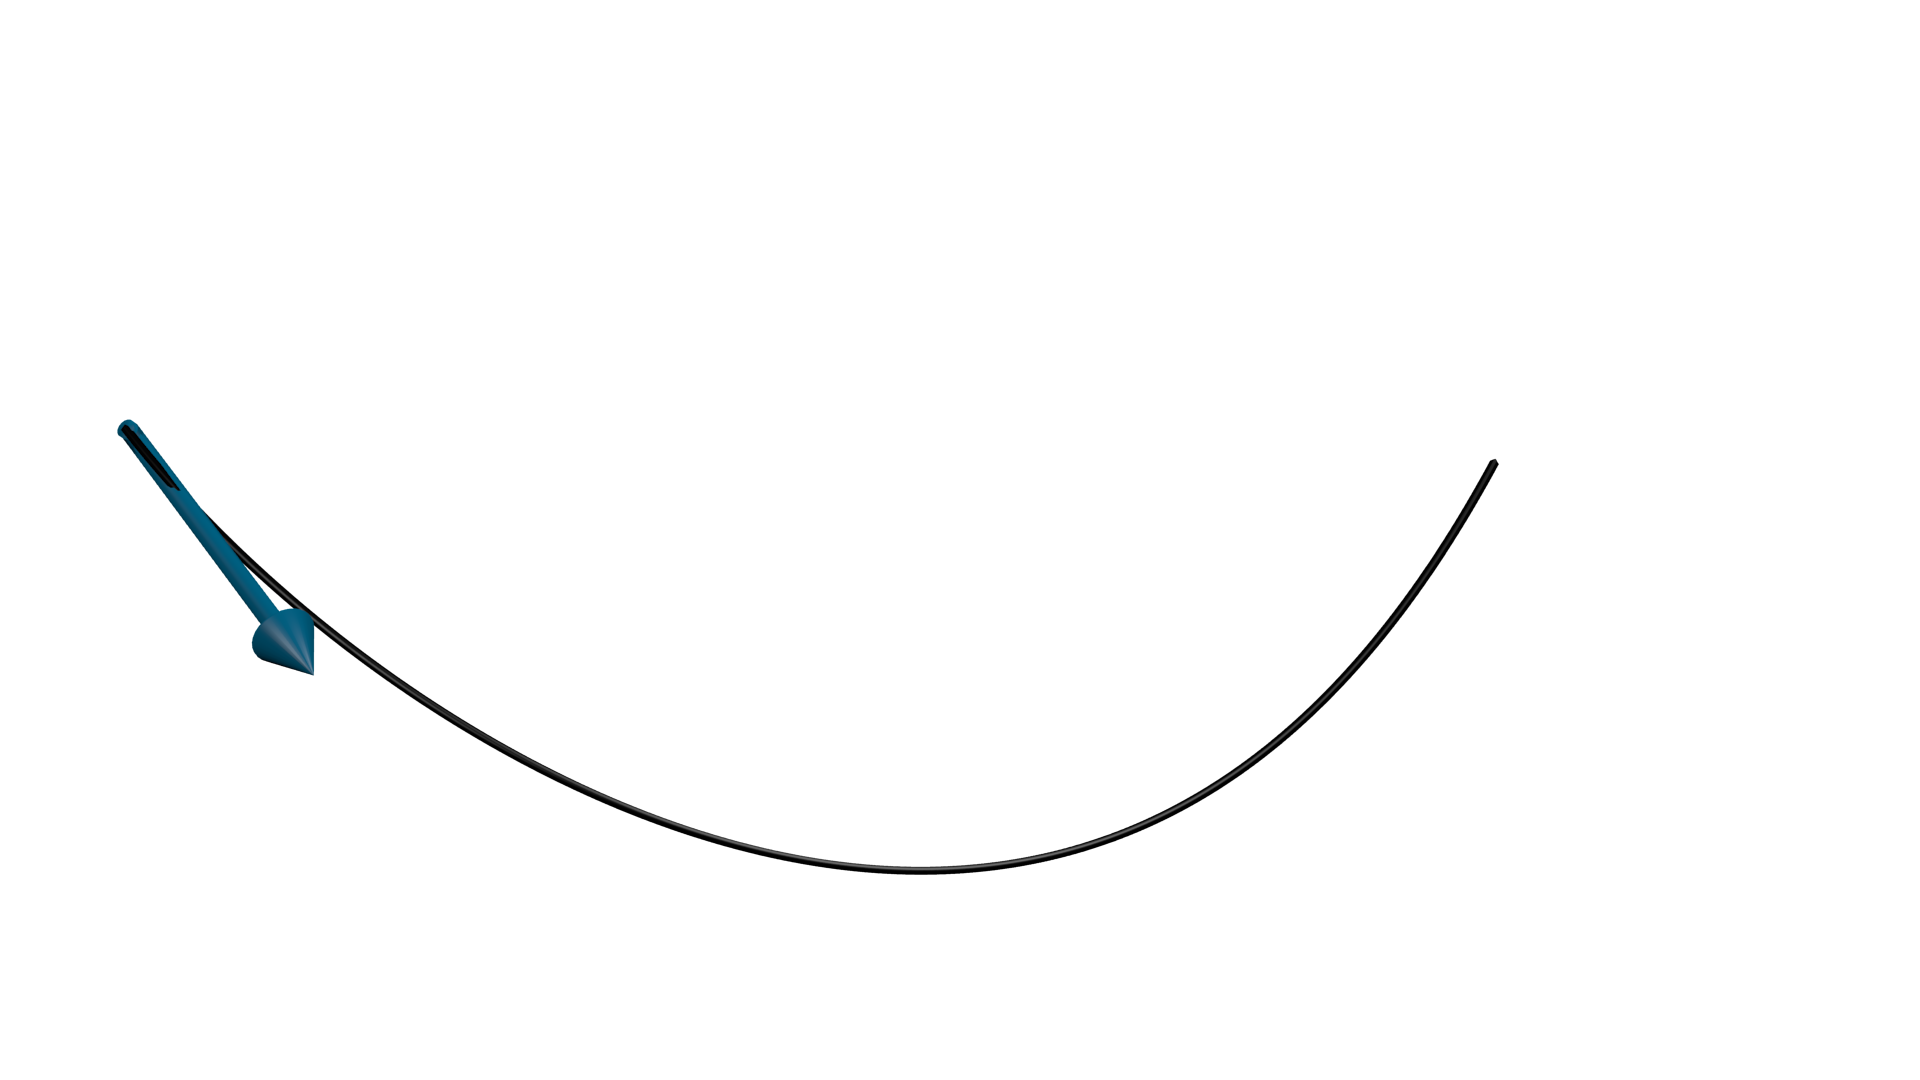
\includegraphics[width=7cm]{../graphics/Frenet_Tan.png}};
            }
            \only<3>{
            \node[inner sep=0pt] (ribbon) at (0,0)
                {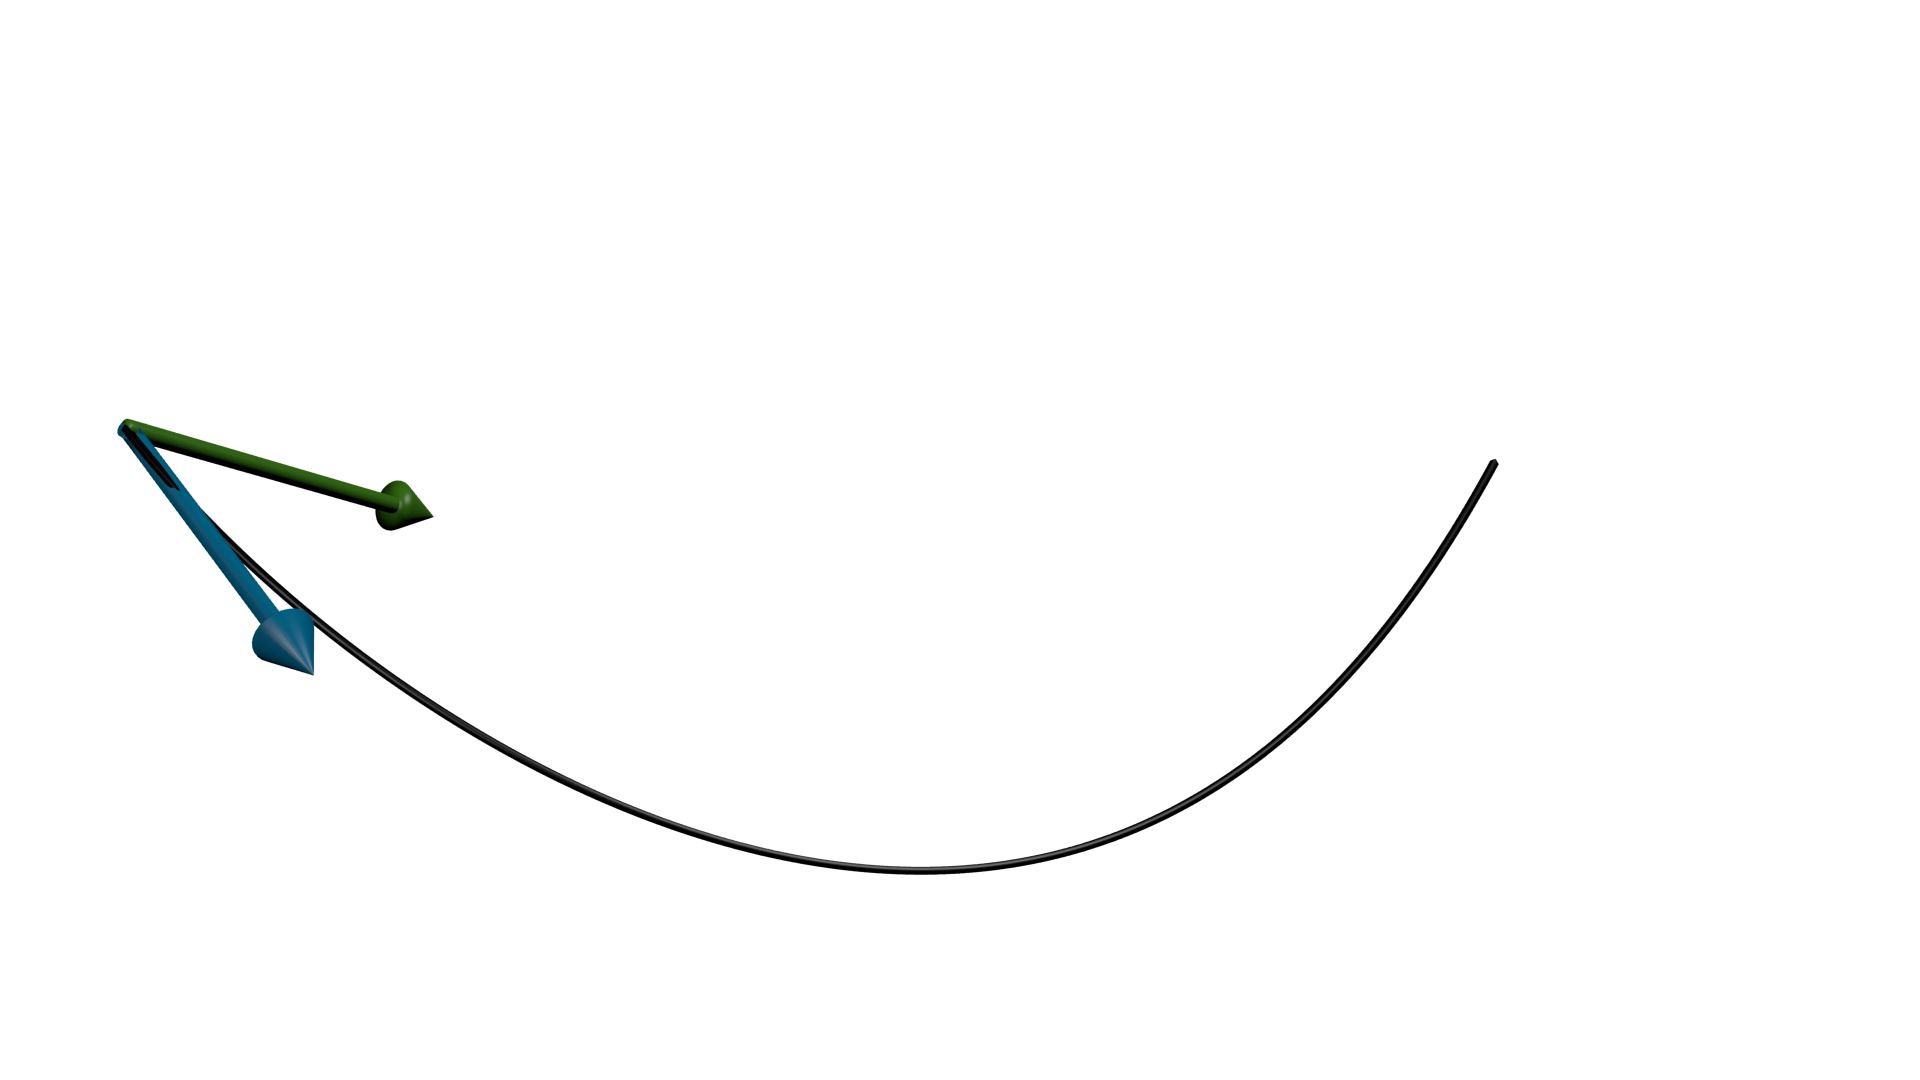
\includegraphics[width=7cm]{../graphics/Frenet_Tan_Nor.png}};
            }
            \uncover<4->{
            \node[inner sep=0pt] (ribbon) at (0,0)
                {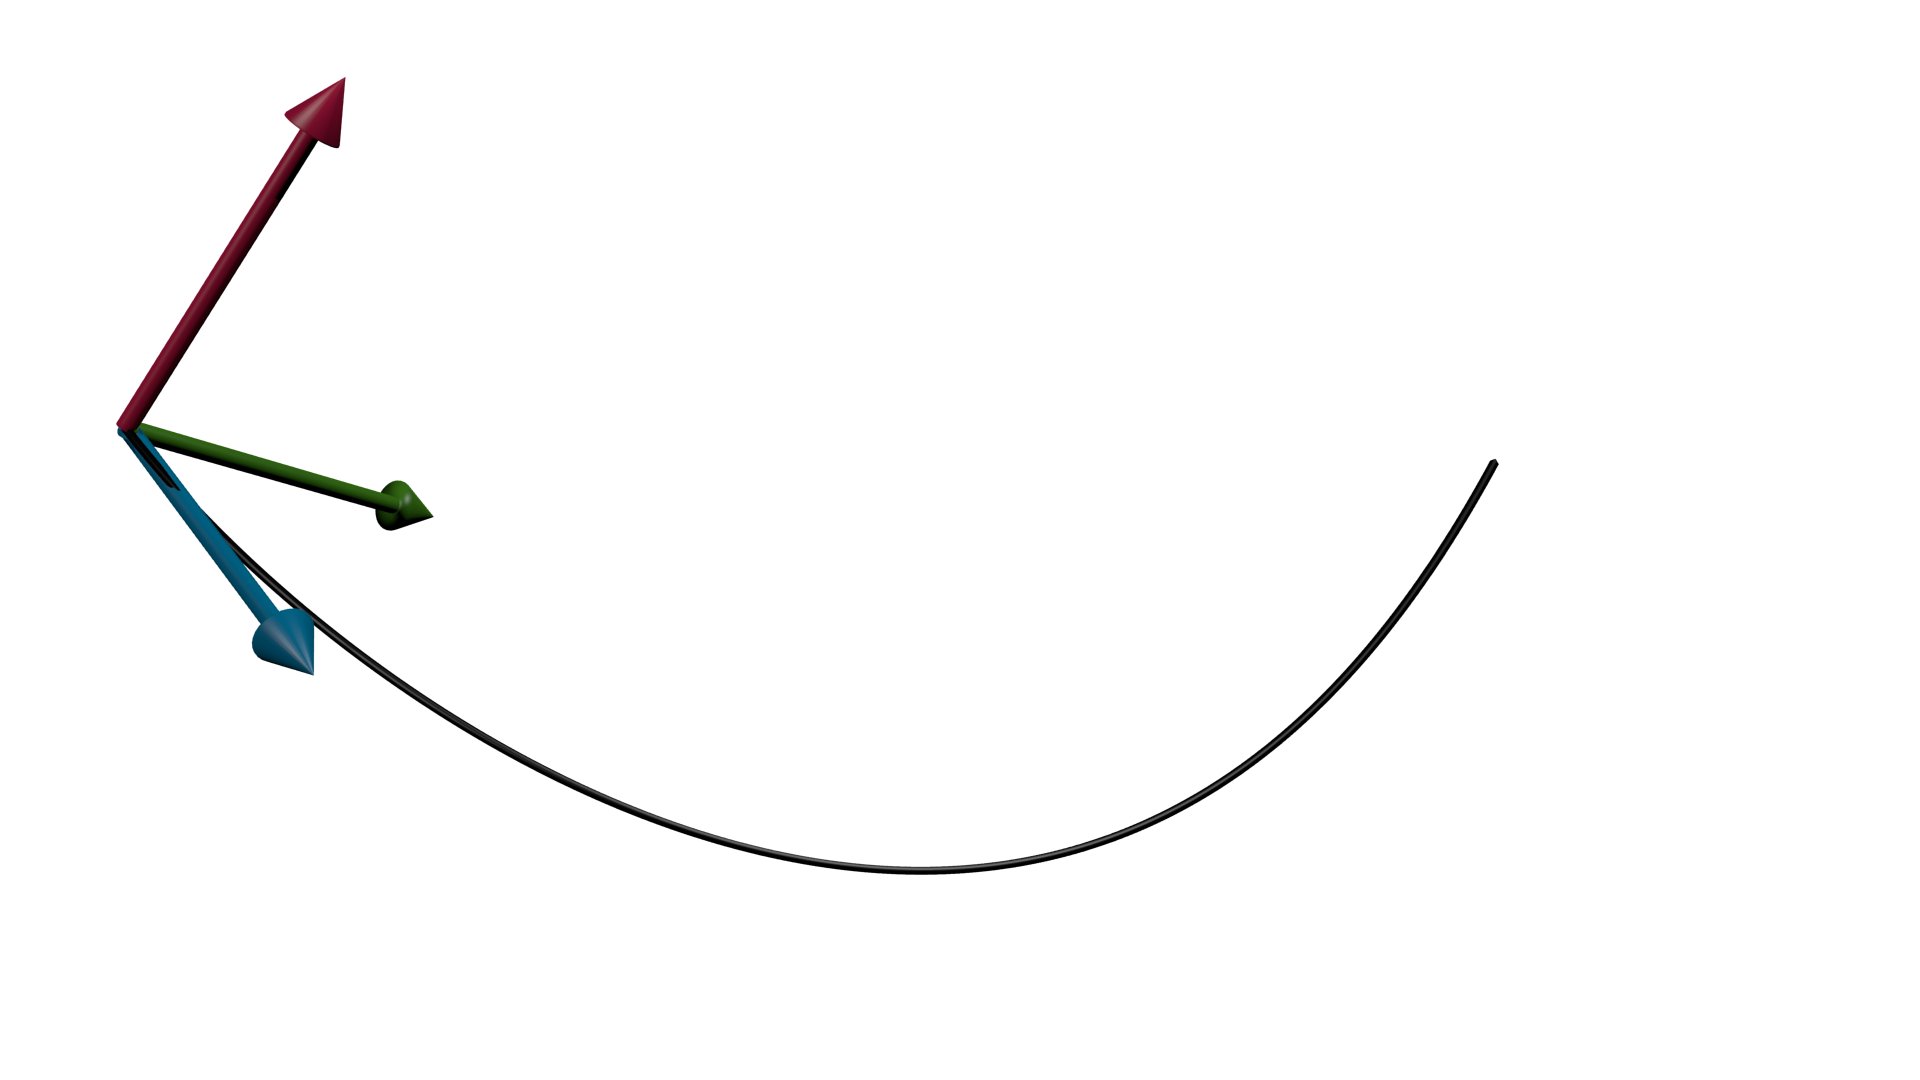
\includegraphics[width=7cm]{../graphics/Frenet_Tan_Nor_Bin.png}};
            }
            \uncover<2->{\node[inner sep=0pt, anchor=east] (C) at ($(ribbon.east) + (-1.4,0.6)$) {$C$};
            \node[inner sep=0pt, anchor= west] (T) at ($(ribbon.west) + (1.2,-0.7) $) {\textcolor{rwthblue}{$T$}};
            }
            \uncover<3->{
            \node[inner sep=0pt, anchor=south] (N) at ($(ribbon.north) + (-1.7,-2)$) {\textcolor{rwthgreen}{$N$}};
            }
            \uncover<4->{
            \node[inner sep=0pt, anchor= south] (B) at ($(ribbon.north) + (-2,-0.3) $) {\textcolor{rwthmagenta}{$B$}};
            }
        \end{tikzpicture}
        \end{column}
      \end{columns} 
      
    \end{Def}
  
    \note{
      %\trickdown %wird manchmal benötigt um den State-Zähler in Frame und Notes zu synchronisieren. Habe noch nicht rausgefunden was der Grund dafür ist.
      \begin{enumerate}
        \item<1-> Bogenl-Param => $|T|=1$
        \item<2-|alert@2> Wir betrachten jetzt Kurven mit pos Krümmung
      \end{enumerate}
    }
  \end{frame}


\end{document}
